%% methods.tex
This chapter describes the methodology used.
A large part of the contribution of this thesis consists of identifying appropriate findings from neuroscience and adapting them to a deep learning setting.
This identified concept and the link between the two disciplines is described in chapter \secref*{neuro_concepts}.
It should be noted that this section presents only one possible interpretation for the implementation of neuroscientific concepts in the context of deep learning and that alternative interpretations might also be promising.
Afterwards, two possible implementation approaches are described, which differ mainly in the type of local self-organisation.
These types of self-organisation are referred to as horizontal and vertical self-organisation and are described in Section \secref*{vertical_self_org} and Section \secref*{horizontal_self_org} respectively.




\section{Neuroscientific Concepts}\seclbl{neuro_concepts}

\subsection{Self-Organisation}\seclbl{neuro_concepts_self_org}
It is known that large parts of the human brain are self-organizing \sidecite{kelso1995dynamic}.
Self-organization is the process by which systems consisting of many units acquire their function through local interaction and without interference from a external supervisory system.
Recently, renowned scientists \sidecite{von_der_Malsburg_Stadelmann_Grewe_2022} put forward the hypothesis that this process of self-organization is \emph{the} key mechanism of natural intelligent systems such as the human brain.
Dresp \sidecite{Dresp2020SevenPO} describes seven clearly identified properties of self-organization in the human brain: (i) modular connectivity, (ii) unsupervised learning, (iii) adaptive ability, (iv) functional resiliency, (v) functional plasticity, (vi) from-local-to-global functional organization, and (vii) dynamic system growth.
However, it is not obvious how these insights from neuroscience can be integrated into a deep learning framework.

Deep learning networks are usually optimized with end-to-end backpropagation of error.
Thus, the entire network is optimized for a specific target.
This is considered a violation of the self-organisation principle, as a global update algorithm (i.e. the optimizer) adjusts all network weights to minimise a global target function.


\begin{claim}
	End-to-end backpropagation of error violates the principle of self-organization. Self-organisation in neural networks requires dividing the network into smaller units that are optimised independently of each other.
\end{claim}

In fact, the plausibility of backpropagation of error for explaining how the brain works was questioned soon after it was published \sidecite{Crick_1989, Grossberg_1987}.
Since then, many alternative and biologically more plausible algorithms have been proposed such as the feedback alignment (FA) algorithm \sidecite{Lillicrap_Cownden_Tweed_Akerman_2014}, generalized recirculation \sidecite{O_Reilly_1996}, as well as target propagation (TP) \sidecite{Le__Cun_1986} (c.f. Section \secref*{alt_train_algo}).
However, Bartunov et al. \sidecite{Bartunov_Santoro_Richards_Marris_Hinton_Lillicrap_2018} have demonstrated that these algorithms do not scale to large vision datasets such as ImageNet \cite{deng2009imagenet} and only work for smaller datasets such as MNIST \cite{MNIST} and CIFAR-10 \cite{cifar_10}.
The only algorithm that seems to scale well is using a proxy objective functions (c.f. Section \secref*{alt_train_algo}).

The biologically most plausible learning algorithm is Hebbian learning (c.f. Section \secref{hebbian}) and its variants such as contrastive Hebbian learning \sidecite{Movellan_1991}.
However, even tough I obtain some promising results in preliminary experiments with Hebbian learning (c.f. Appendix \chref{exp_hebb_learning}), this algorithm doesn't seem to be well suited to learn good image representation if a network is trained from scratch.

Thus, the use of proxy objective functions\sidenote{proxy objective functions are loss functions that are only applied to local units of a system} seems promising; the updates of weights are done in separate local units, yet the power of current deep learning training algorithms can be exploited and systems can be created that can solve complex problems and scale to large datasets by interacting with each other.

\begin{implementation}
	Instead of using end-to-end backpropagation of error to optimise the whole system according to a single global objective function, proxy objective functions are applied to local units. Thus, self-organisation takes place through the optimisation of local units instead of an overall system.
\end{implementation}

The next ambiguity is what local units are in a deep learning setting.
In deep learning models, typically not neurons are modelled but the trainable parameters\sidenote{the weights $\boldsymbol{w}$ and the bias $\boldsymbol{b}$ are modelled, so that the output $y$ can be calculated as $\boldsymbol{y}=\boldsymbol{w} \cdot \boldsymbol{x} + \boldsymbol{b}$ for given data $\boldsymbol{x}$}.
One of the strengths of deep learning systems is that matrix multiplications allow to calculate the layer outputs in one step.
Calculating each neuron activity separately, on the other hand, would be very inefficient.
Therefore, the smallest meaningful unit for local updates seems to be a layer and not a single neuron.
If a neural network is visualised layer-wise from left to right, then the self-organising units line up horizontally. This is why layer-wise self-organisation is also referred to as ``horizontal self-organisation'' in this thesis (c.f. Figure \figref*{horizontal_vertical_self_org}).

\begin{implementation}
	Self-organisation takes place within local units. A local unit can be a part of a model such as layer.
	In this thesis, this type of self-organisation is called horizontal self-organisation.
\end{implementation}

\begin{figure}[h]
    \centering
    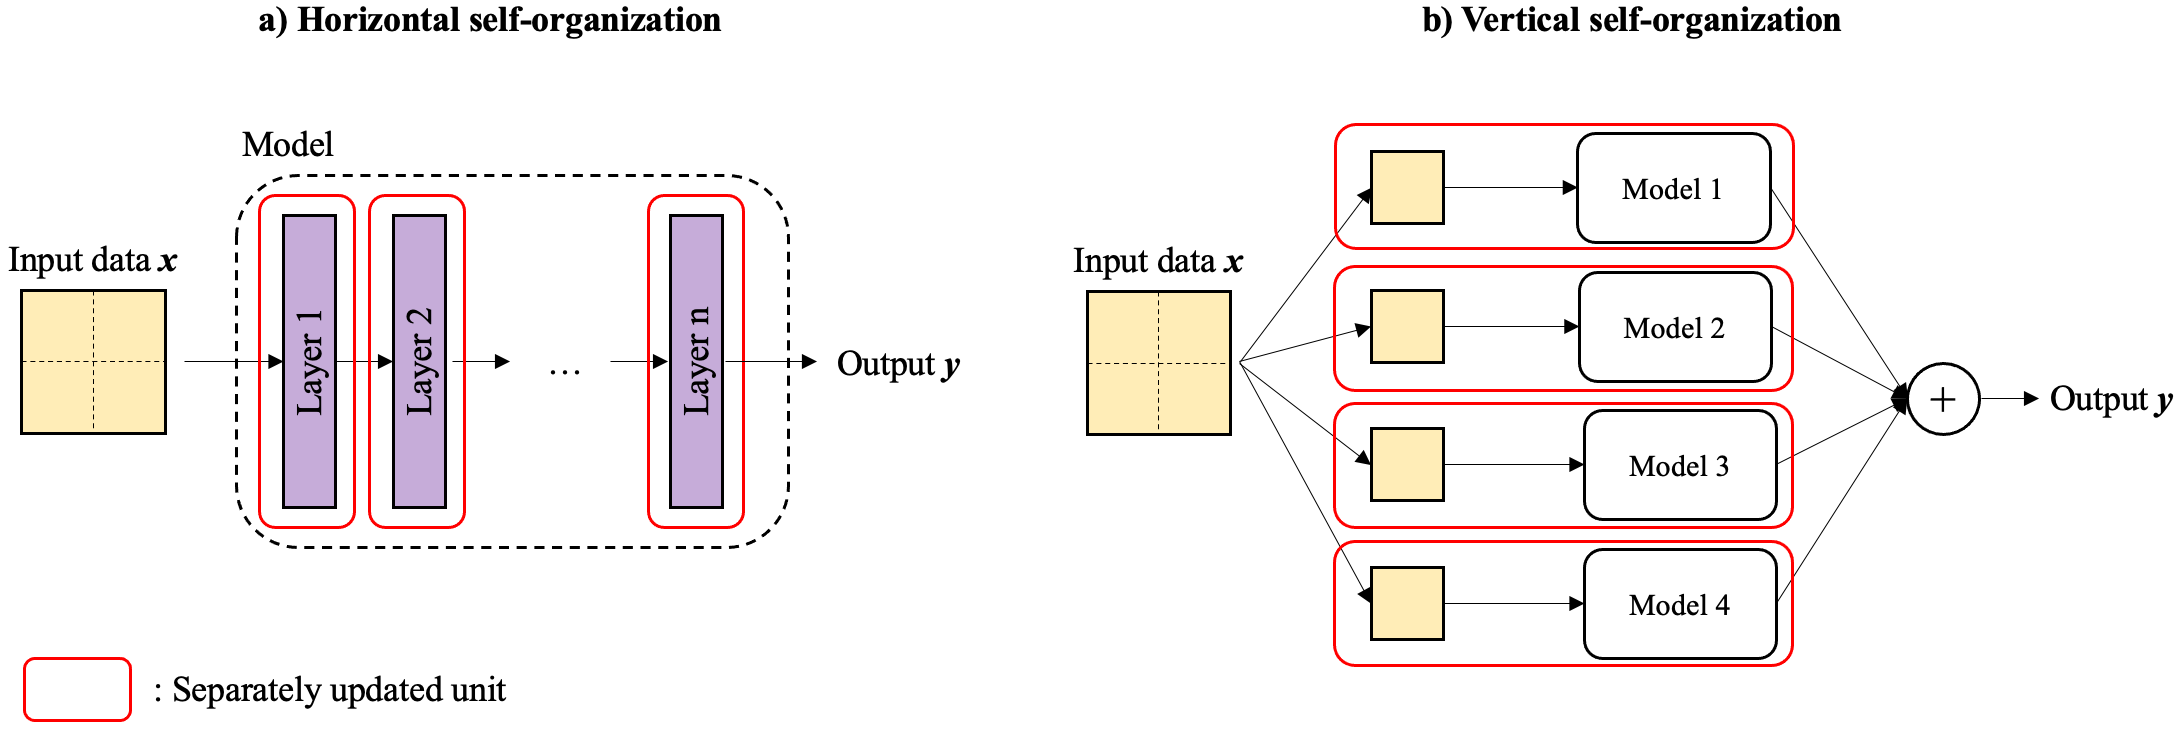
\includegraphics[width=0.99\textwidth]{horizontal_vertical_self_org}
    \caption[Overview of horizontal and vertical self-organization]{Two different ways of building self-organizing units. Self-organization can either take place horizontally (i.e. layer-wise) within a model (a) or vertically by splitting the data into patches and processing them with independent units (b). The independent units are marked with a red frame.}
    \figlbl{horizontal_vertical_self_org}
\end{figure}
 
A second type of self-organisation is not to split the model into separate units but to split the data.
The input data can be divided into smaller patches and then be processed by independent models.
It is important that one model does not process the entire set of existing patches, as is the case with the vision transformer. If only one model is used, there would again be an end-to-end backpropagation of error on a single unit.
But if the patches are processed by a graph of independent models, then each model can be considered as a self-organising unit.
In this thesis we call this kind of self-organisation the ``vertical self-organisation'' (c.f. Figure \figref*{horizontal_vertical_self_org}).

\begin{implementation}
	A second type of self-organising unit can be a model that processes a subset of input data that is not shared with other models. In this thesis, this type of self-organisation is called vertical self-organisation.
\end{implementation}


\subsection{Net-Fragments}\seclbl{neuro_concepts_net_fragments}
Another very important principle according to von der Malsburg et al. \cite{von_der_Malsburg_Stadelmann_Grewe_2022} is that neurons form net-fragments (a.k.a. sub-networks) that represent features of objects (c.f. section \secref{natural_intelligence}).
For example, some net-fragments may represent shapes and structures while a multitude of such net-fragments together represent objects such as persons or entire scenes.
Net fragments are a compositional data structure, meaning that some low-level features can be composed to a higher-level feature and multiple higher-level features are composed to an object.
To some extend, neural networks do this as well; data is fed into the network, the first layer extract some low-level patterns, and subsequent layer combine these patterns in higher-level features in a hierarchical manner.
However, there is one big difference: The features that are used to fulfil a specific task such as classification are extracted from the latent space of \emph{one} single layer.
Net-fragments in the human brain, on the other hand, are not considered to be present at a specific point in time but to be built up over a short period of time.

\begin{claim}
	Net fragments are represented by groups of neurons and their activity over multiple time-dependent spikes. In addition, several net fragments can be composed into a higher-level fragments. Thus, objects are not represented by a single neuron but by all neurons that were activated due to this object.
\end{claim}

Deep learning models are not based on time-dependent spikes of neurons that compose features to more complex features.
However, a time-step could be interpreted as a forward-step from one layer to the next within a network of layers.
Thus, net-fragments would be the activation of multiple layers.
This interpretation is also in line with the compositional property of net-fragments.
Low-level features that are detect within the first layers activate higher-level features in subsequent layers.
An object, however, is not represented in the last layer of a neural network but through all activations within the network.
Thus, representations of objects cannot be extracted from a single layer but from multiple layers.
Intuitively, this seems promising.
For example, auto-regressive models applied on speech capture different information at different layers of the network \sidecite{Chung_Hsu_Tang_Glass_2019}.
While the first layers contain more information to distinguish speakers, representations in later layers provide more phonetic content.
Thus, extracting information from several layers could lead to representations containing more information.

\begin{implementation}
	Net-fragments cannot be extracted from one single layer. Therefore, the representations of an image are extracted from multiple layers.
\end{implementation}

In the human brain, distinct groups of neurons represent specific net fragments.
This means that neurons are only active when the corresponding feature is present in the input and are inactive otherwise.
Moreover, the features represented by the neurons should be meaningful\sidenote{interpretable in the sense that a neuron is active if a specific feature is present and inactive otherwise} and consequently not active for every existing object.
This inevitably leads to the sparse and diverse activations.
The activations are sparse and diverse because, the object in the image consists of only a small sub-set of all learned features. Thus, only a small sub-set of the neurons should be active for a given object.
When the input changes and a different object is shown to the model, also the set of active neurons should change.

\begin{claim}
	The activation patterns of neurons that represent net-fragments must be sparse and diverse to obtain meaningful activation patterns.
\end{claim}

The extent to which neuronal networks contain or can produce net fragments with meaningful activation patterns is investigated in detail in a preliminary study.
The methodology used as well as an in-depth evaluation is described in the appendix in the Chapter \chref{net_fragments}.
In summary, it was found that neural networks do not contain net fragments with meaningful activation patterns by default. Typically, there are neurons that are always active regardless of the input data and encode most of the input information in their activation strength.
Other neurons, however, are never active and are therefore not needed by the network.
If, on the other hand, a sparsity and diversity constraint is applied, then layers are obtained with neurons that appear to be suitable for net fragments.

\begin{implementation}
	Sparse and diverse activation patterns can be obtained by imposing sparsity and diversity constraints to the objective function of the model.
\end{implementation}

However, sparsity and diversity constraints are mainly necessary to obtain meaningful and more robust activation patterns.
They don't seem to be necessary, for example, if the goal is to obtain good classification performance.
An alternative that lead also to robust and meaningful activations is to model the net-fragments as probability distribution.
For example, variational autoencoders (c.f. Section \secref*{visual_rep_learning}) model their latent space as a multivariate Gaussian distribution.

%Especially for models based on horizontal self-organisation, it seems important to impose these constraints on all layers.
%For models with vertical self-organisation, on the other hand, these constraints do not need to be applied to all layers, as long as there are enough models that can only see very small input patches. In this case, a sub-model can only recognise a very spatially-limited feature, which corresponds to a low-level feature. In order to recognise higher-level features or whole objects, interaction with neighbouring sub-models is necessary.
%Thus, net-fragments are composed over several sub-models.
%In this case, it is sufficient to impose the constraints to the function that composes the the representation of the sub-models to higher-level net fragments or to objects.

\subsubsection{Sparsity}
Sparistiy seems to be an important principle in biological networks.
Presumably, this is because the neurons in the brain can be inhibitory or excitatory by firing spikes at different time intervals. An artificial neuron, on the other hand, uses a floating point number as its state and can thus represent an infinite number of different states, in contrast to the biological neuron.
Thus, an artificial neuron is able to represent many different things while the biological neuron is responsible for specific features.
Therefore, the activations of biological neurons \emph{must be} sparse, while the activations of artificial neurons \emph{do not have to be} sparse (but being sparse has also advantages for artificial neurons, see below).

Sparsity is deeply embedded in the biological learning process.
For example, in the visual cortex of mice are more than 75\% of the neurons active before the first opening of the eyes, 36\% after the opening of the eyes and only 12\% in adulthood \sidecite{Rochefort_Garaschuk_Milos_Narushima_Marandi_Pichler_Kovalchuk_Konnerth_2009}.
Thus, a sparsification of neuronal activations takes place through visual experience.
In the field of deep learning, sparsity is often interpreted in two different forms; sparse weight matrices and sparse activation matrices.
Sparse weight matrices are often chosen to make models smaller or to increase inference speed \sidecite{Louizos_Welling_Kingma_2018, Hoefler_Alistarh_Ben_Nun_Dryden_Peste_2021}.
From a biological point of view, this process of first creating a large network and then shrinking it is obviously not plausible\sidenote{otherwise we would have a large brain at the beginning, which becomes smaller by factors in the course of time}.
Sparse activations, on the other hand, can increase robustness \cite{Panousis_Chatzis_Theodoridis_2021}.
Intuitively, sparse activations enforce that only the most relevant information is passed to the subsequent layer.
Furthermore, combining sparsity with diversity can help to obtain more interpretable activations (c.f. Appendix Chapter \chref*{net_fragments}).

\subsection{Lateral Connections}\seclbl{neuro_concepts_lateral_connections}
In addition to forward connections, lateral connections are also located in visual cortex \sidecite{gilbert1990lateral}.
Thus, the biological neurons are not only connected to the neurons in the subsequent layer but also within the same layer.
Von der Malsburg et al. \cite{von_der_Malsburg_Stadelmann_Grewe_2022} describe that lateral connections help active neurons to support each other in order to remain active:
Initially, many neurons are active, but relatively quickly a part of the neuron becomes inactive and only those neurons that support themselves remain active. In this way, lateral connections can lead to the emergence of high-level features from initial activations.

\begin{claim}
	Lateral connections allow active neurons to support each other and to remain active.
\end{claim}


Neural networks lack this time dynamic and neurons do not suddenly become inactive during a forward pass. 
In addition, initial experiments have shown that performance does not improve when the activation maps of neural networks are sparsified over several steps.
One assumption is that all information is already contained in the data at the beginning and the same sparsified activations can also be generated in one initial step.

However, the lateral support between neurons seems promising if the input changes slightly:
An activation map can be calculated for a given input image. In a next step, the input can slightly be changed through data augmentation to btain another activation map from the same image. Thus, the network receives different views of the same image and generates different activation maps of the same image. In every step, the model can decide whether the activation map from the previous step was correct or if the activation map should be updated.

\begin{figure}[h]
    \centering
    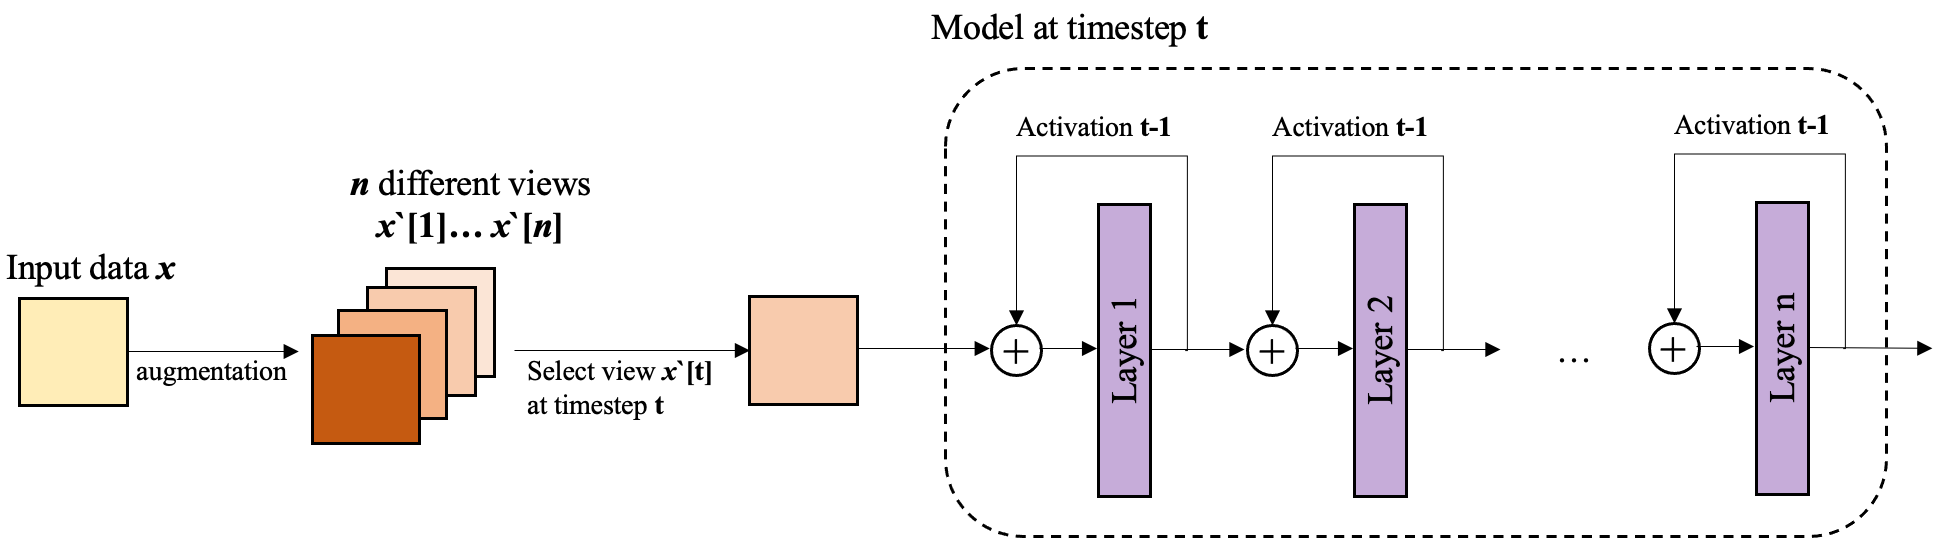
\includegraphics[width=0.99\textwidth]{lateral_connections}
    \caption[Illustrative network architecture of a model with lateral connections]{An illustrative network architecture of a model with lateral connections: An in sample $x$ is augmented $n$ times to obtain $n$ different views $x'[1], ..., x'[n]$ of the same sample. At every timestep $t$, the sample $x'[t]$ is fed through the model. Each layer receives the activation map of the previous layer as input as well as its own activation maps from the previous time-step $t-1$.}
    \figlbl{lateral_connections}
\end{figure}

This could be implemented by interpreting the lateral connection as a recurrent connection.
An illustrative architecture of such a model is shown in Figure \figref{lateral_connections}.
A data sample $x$ can be augmented with data augmentation methods $n$ times to obtain $n$ different views $x'[1], ..., x'[n]$ of the input sample.
Afterwards, the $n$ views are iteratively fed into the model.
At every time-step $t$, the model calculates an activation map $a_l[t]$ for each layer $l$.
If $t>1$, the input of the layer $l$ is not only the activation map of the layer $l-1$ but also the activation map of the previous time-step $a_l[t-1]$.
The activation map of the previous time-step is stored $a_l[t-1]$ by the recurrent (lateral) connection.
Thus, the activation map $a_l[t]$ is not only calculated based on the activation map of the previous layer $a_{l-1}[t]$ but also based on the activation map of the previous time-step $a_l[t-1]$.
This allows each layer to preserve the activation map $a_l[t-1]$ from the previous time-step or to correct it based on a slightly different input $a_{l-1}[t]$ from the previous layer. The lateral connections thus support the activations within a layer; a layer can look at several inputs and decide which features are present over several time-steps (support these features over several time-steps).

\begin{implementation}
	A lateral connection can be implemented as a recurrent connection that ``stores'' the layer's activation of a previous time-step.
	If the same input is present for several time-steps in a slightly augmented version, the layers can keep their previous activation maps (lateral support) or correct them.
\end{implementation}

With vertical self-organisation, the lateral connections can be implemented not only as recurrent connections within layers, but also as connections between the sub-models.
In this case, each sub-model extracts a distinct low-level feature.
Based on this feature, a guess can be made to which higher-level feature or object the extracted feature belongs to.
Through communication with neighbouring sub-models, this guess can either be supported or rejected.
Thus, the lateral connections are used as a ``support channel'' between sub-models. 

\begin{implementation}
	In the case of vertical self-organisation, a lateral connection can be implemented as connection between sub-models to vote for which high-level feature or object is represented in the image. Either the prediction of a model can be supported by neighbouring models or rejected.
\end{implementation}


\subsection{Other Principles}\seclbl{neuro_concepts_others}
Other important principles that are considered promising are a \emph{continuous input} signal and an \emph{embodiment} of the agent.
However, implementing such an interaction between an agent and an outside world is out of scope for this thesis but might be interesting for future work.

The visual cortex receives a continuous input signal.
This allows the tracking of moving objects and enables an object to be perceived from different angles. Since the change of the object between the captured frames is small, it can be determined that it is always the same object instance and consequently mapped to the same mental object prototype of a world model.

An ANN, on the other hand, is typically trained on samples that have little relation to each other.
When the system is trained on images, each frame is different; with videos, each sequence of frames is different.
A continuous input might help to get better representation of objects through self-supervised learning.
If an input is continuous and shows the same object from different angles or in different transformations (e.g. stretching) and it can be inferred that it is the same object then the object representations derived from this continuous stream can be homogenized.
These principles are already applied to some extent by self-supervised learning systems for computer vision.
In contrastive learning, a popular form of self-supervised learning, two different views are derived from one image by data augmentation, and their representations are then pushed closed together in the feature space \sidecite{chen2020simple, chen2020big, caron2020unsupervised}.
However, this paradigm is still quite limited since only two views of the same scene and not the continuous transformation of an object are presented to the learning system.

\begin{claim}
	A continuous input stream can help to build a better representation of objects, especially if the objects are slightly transformed between captured frames or if the point of view changes continuously and smoothly.
\end{claim}


Furthermore, efference copies of motor signals in the form of neuronal activities are directly sent to the brain’s sensory system if animals are moving \sidecite{Keller_Bonhoeffer_Hübener_2012}.
Such efference copies can be useful to better understand objects and how they behave when undergoing object transformations.
To do so, the agent must be allowed to perform actions and interact with its world.
This gives the agent more information about the objects but also about the physical properties of a (virtual or real) world. For example, he can perform different actions on different objects: He can rotate, squeeze, stretch or move objects. By doing so, he receives different visual and sensory feedback for identical actions on different objects.
The agent can map the captured feedback signals to the object representations of an internal world model.

Furthermore, the agent can learn to understand objects better by improving his internal object representations on its own. For example, if the agent examines an object and his current internal object representation does not describe how the object looks from the side, then the agent can rotate the object accordingly and complete or correct the representation. 
Such a behaviour could be implemented within the agent itself, for example, by optimising an entropy-based loss in order that the agent explores the world and tries to learn unknown things \sidecite{storck1995reinforcement, Rybicka_Schraudolph_Schmidhuber_2001}.


\begin{claim}
	Allowing an agent to interact with the world can help to learn better object representations and to build a better world model.
\end{claim}



% TODO: target function und objective function vereinheitlichen
% TODO: net-fragment or net fragment




\section{Vertical Self-Organization}\seclbl{vertical_self_org}
2 Arten von Loss: 1x Diversity + Sparsity, 1x MI zwischen vorherigem und nachfolgendem Layer

\section{Horizontal Self-Organization}\seclbl{horizontal_self_org}